%%%%%%
%$Autor: Wings $
%$Projekt: $
%$Dateiname:Mosfet.tex$
%$Beschreibung: Erläuterung des Mosfets$
%%%%%%

\chapter{Mosfet-Modul mit Grove-Schnittstelle}\label{GroveMosfet-Modul}

\section{Einleitung}
Das Grove-Mosfet-Modul ist ein einfach integrierbares Bauteil, das die Steuerung von hohen Leistungen mittels eines Mikrocontroller-Signals ermöglicht.\ref{fig:Mosfet} Mosfets sind Schlüsselkomponenten in modernen elektronischen Schaltungen, die als Verstärker oder Schalter eingesetzt werden. Das Grove Mosfet-Modul nutzt diese Technologie, um die Ansteuerung leistungsintensiver Lasten wie LED-Streifen, Motoren oder andere hohe Ströme benötigende Komponenten zu vereinfachen.
Das Modul ist Teil des Grove-Systems, das sich durch seine Modularität und einfache Anschlussmöglichkeiten auszeichnet. Es bietet Entwicklern eine unkomplizierte Methode zur Integration des Mosfets in das Projekt, ohne die Komplexität diskreter Transistor-Schaltungen aufbauen zu müssen. Durch die Verwendung von Steckverbindungen und vorgefertigten Sensoren und Modulen können Entwickler schnell und effizient prototypische Lösungen sowohl im industriellen als auch im Hobbybereich umsetzen.
\cite{GroveGuide2023}

\section{Funktionsweise}
Das Grove Mosfet-Modul nutzt den Mosfet als elektronischen Schalter, der durch ein Steuerungssignal vom Mikrocontroller aktiviert wird. Sobald das Signaleingang eine festgelegte Spannung überschreitet, wird der Mosfet leitend und ermöglicht den Stromfluss zwischen Source und Drain. Diese Eigenschaften erlauben es, hohe Spannungen und Ströme zu regulieren, die nicht direkt vom Mikrocontroller geschaltet werden können. Außerdem bietet der Mosfet  eine schnelle Schaltgeschwindigkeit und eine hohe Effizienz durch seine geringe Verlustleistung im leitenden Zustand.
\cite{MOSFETApplication2018}

\section{Technische Spezifikationen}
Die folgende Tabelle \ref{tab:Mosfet} zeigt die wichtigsten Spezifikationen des Grove Mosfet-Moduls:

\begin{table}
	\centering
	\caption{Technische Daten: Grove Mosfet-Modul 
	\cite{GroveGuide2023}}
	\label{tab:Mosfet}
	\begin{tabular}{|l|p{8cm}|}
		\hline
		Mosfet-Typ & BSS138 \\
		\hline
		Gate-Threshold-Spannung & 2-4 V \\
		\hline
		Maximaler Durchlass-Strom & 500 mA \\
		\hline
		Maximaler Drain-Source-Spannung & 50 V \\
		\hline
		Abmessungen & 40 mm x 20 mm \\
		\hline
		Schnittstelle & Grove Connector \\
		\hline
		Betriebstemperatur & -40 bis 85°C \\
		\hline
	\end{tabular}
\end{table}

\begin{figure}
	\centering
	
\includegraphics[width=0.7\linewidth]{Mosfet/MosfetGrove}
	\caption{Grove Mosfet\cite{GroveMOSFETDocs}}
	\label{fig:Mosfet}
\end{figure}


\section{BSS138 als Schalter}
Der BSS138 ist ein N-Kanal-Mosfet mit niedriger Gate-Schwellspannung, der sich ideal als Schalter in Mikrocontroller-Schaltungen eignet. Wird am Gate eine Spannung über der Schwellspannung angelegt, leitet der Transistor zwischen Drain und Source, wodurch er als elektronischer Schalter fungiert. Die Abbildung \ref{fig:Mosfet-schaltplan} soll die Funktionsweise weiter veranschaulichen. Der BSS138 ermöglicht es beispielsweise, Aktoren wie LEDs oder andere Verbraucher über die digitalen Ausgangspins eines Mikrocontrollers zu steuern, ohne diese direkt zu belasten. Aufgrund seiner geringen Gate-Kapazität ist der BSS138 auch für schnelle Schaltvorgänge geeignet \cite{nexperiabss138}.

\begin{figure}
	\centering
	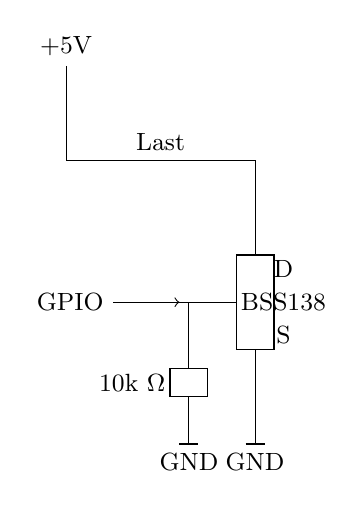
\begin{tikzpicture}[scale=1.2, every node/.style={font=\small}]
		
		% +5V und Last
		\draw (0,4) node[above]{+5V} -- (0,3.5);
		\draw (0,3.5) -- (0,3);
		\draw (0,3) -- (2,3) node[midway, above]{Last};
		\draw (2,3) -- (2,2.2);
		
		% Mosfet  (symbolisch)
		\draw (2,2.2) -- (2,2);
		\draw (1.8,2) rectangle (2.2,1);
		\node at (2.3,1.85) {D};
		\node at (2.3,1.15) {S};
		\node at (2.3,1.5) {BSS138};
		
		\draw (2,1) -- (2,0.5);
		\draw (2,0.5) -- (2,0) node[below]{GND};
		
		% Gate-Anschluss
		\draw (1.8,1.5) -- (1.2,1.5);
		\draw[<-] (1.2,1.5) -- (0.5,1.5) node[left]{GPIO};
		
		% Pulldown-Widerstand
		\draw (1.3,1.5) -- (1.3,0.8);
		\draw (1.1,0.8) rectangle (1.5,0.5);
		\node at (0.7,0.65) {10k $\Omega$  };
		\draw (1.3,0.5) -- (1.3,0) node[below]{GND};
		
		% Massezeichen unter Source
		\draw (1.9,0) -- (2.1,0);
		\draw (1.2,0) -- (1.4,0);
		
	\end{tikzpicture}
	\caption{Elektrischer Schaltplan eines Mosfets nach \cite{nexperiabss138}}
	\label{fig:Mosfet-schaltplan}
\end{figure}




\section{Anwendungen}
Das Grove Mosfet-Modul ist ideal für Anwendungen, die eine Steuerung von höheren Lasten oder die Regelung von Gleichspannungskomponenten benötigen. Häufige Einsatzbereiche sind:

\begin{itemize}
	\item \textbf{LED-Beleuchtung}: Steuerung von LED-Streifen oder Gruppen, um unterschiedliche Beleuchtungseffekte zu erzielen.
	\item \textbf{Motorsteuerung}: Aktivierung und Regelung von Gleichstrommotoren für einfache Antriebslösungen.
	\item \textbf{Energieverwaltungssysteme}: Schalten und Verwalten von verschiedenen Stromkreisen basierend auf elektronischen Eingabeparametern.
	\item \textbf{Heizelemente}: Einsatz in Heizbettansteuerung von 3D-Druckern.
\end{itemize}

Die Modularität und einfache Handhabung des Grove Mosfet-Moduls stellt sicher, dass es sowohl für Anfänger als auch für erfahrene Entwickler geeignet ist, die schnell und effizient Leistungsschaltungen in ihren Projekten integrieren möchten.\cite{GroveMOSFETDocs}

\section{Einfache Anwendung} \label{Test:Mosfet Solenoid}
Das Programm \ref{Code:Mosfet} ermöglicht es das Mosfet über Pulsweitenmodulation (PWM) mit einem Arduino anzusteuern. Es wechselt zwischen festen Geschwindigkeiten und einer kontinuierlichen Beschleunigung und Verzögerung, um die Funktion des Mosfets als elektronischer Schalter zu veranschaulichen. Dabei wird der PWM-Ausgang D12 verwendet, um das Modul zu steuern. Für den ersten Test ist das Mosfet über ein Grove-Kabel mit dem Tiny-ML-Shield verbunden, verwendet wird der Stecker J1 \ref{fig:TML_Cam} am Tiny-ML-Shield. Die Stromversorgung erfolgt über ein 5V Netzteil \ref{tab:Mosfet-connections} an den Schraubklemmen (gekennzeichnet mit \ac{vin} und GND). Zum Testen wird das Solenoid an den Schraubklemmen Befestigt (gekennzeichnet mit Out und GND). Der Code schaltet dann das Solenoid \ref{Code:Mosfet}. Der Schließer sollte vor und zurück bewegt werden.



\begin{figure}
	\centering
	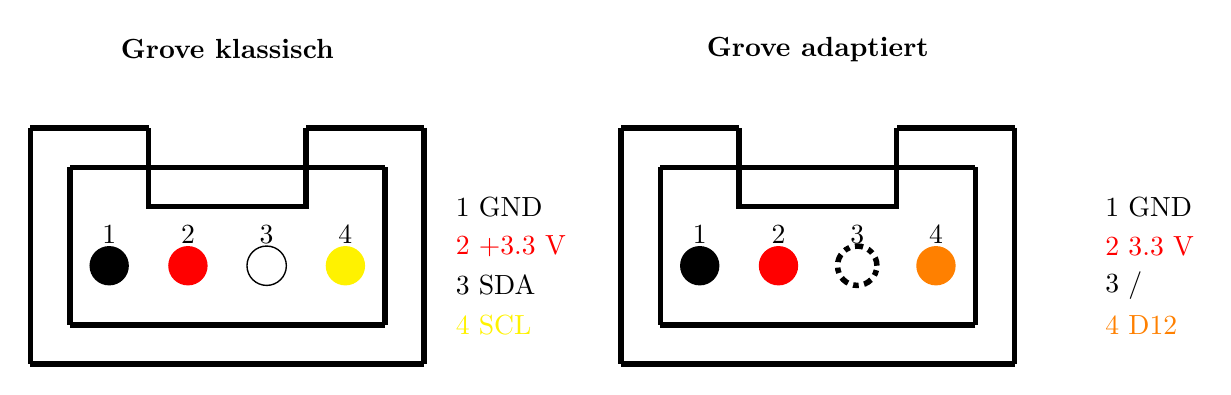
\begin{tikzpicture}[line width=2pt]
		
		% ----- Grove klassisch -----
		\node at (2.5,4) {\textbf{Grove klassisch}};
		
		% Steckerform
		\draw (0,0) -- (5,0);
		\draw (0,3) -- (0,0);
		\draw (0,3) -- (1.5,3);
		\draw (1.5,2.5) -- (1.5,3);
		\draw (1.5,2.5) -- (0.5,2.5);
		\draw (0.5,0.5) -- (0.5,2.5);
		\draw (0.5,0.5) -- (4.5,0.5);
		\draw (5,0) -- (0,0);                         
		\draw (5,3) -- (5,0);                         
		\draw (5,3) -- (3.5,3);                       
		\draw (3.5,2.5) -- (3.5,3);                   
		\draw (3.5,2.5) -- (4.5,2.5);                 
		\draw (4.5,0.5) -- (4.5,2.5);                 
		\draw (4.5,0.5) -- (0.5,0.5);
		
		% Mittleres Rechteck
		\draw (1.5,2.5) rectangle (3.5,2);
		
		% Pins klassisch neu angeordnet: 1=GND, 2=3.3V, 3=SDA, 4=SCL
		\fill[black] (1,1.25) circle[radius=0.25];    % GND
		\fill[red] (2,1.25) circle[radius=0.25];      % 3.3 V
		\draw[fill=white, draw=black, line width=0.5pt] (3,1.25) circle[radius=0.25]; % SDA
		\fill[yellow] (4,1.25) circle[radius=0.25];   % SCL
		
		% Pinnummern
		\node at (1,1.65) {1};
		\node at (2,1.65) {2};
		\node at (3,1.65) {3};
		\node at (4,1.65) {4};
		
		% Beschriftung rechts
		\node[black, anchor=west] at (5.25,2) {1 GND};
		\node[red, anchor=west] at (5.25,1.5) {2 +3.3~V};
		\node[black, anchor=west] at (5.25,1) {3 SDA};
		\node[yellow, anchor=west] at (5.25,0.5) {4 SCL};
		
		% ----- Grove adaptiert -----
		\begin{scope}[xshift=2.5cm]
			
			\node at (7.5,4) {\textbf{Grove adaptiert}};
			
			% Steckerform
			\draw (5,0) -- (10,0);
			\draw (5,3) -- (5,0);
			\draw (5,3) -- (6.5,3);
			\draw (6.5,2.5) -- (6.5,3);
			\draw (6.5,2.5) -- (5.5,2.5);
			\draw (5.5,0.5) -- (5.5,2.5);
			\draw (5.5,0.5) -- (9.5,0.5);
			\draw (10,0) -- (5,0);                         
			\draw (10,3) -- (10,0);                         
			\draw (10,3) -- (8.5,3);                       
			\draw (8.5,2.5) -- (8.5,3);                   
			\draw (8.5,2.5) -- (9.5,2.5);                 
			\draw (9.5,0.5) -- (9.5,2.5);                 
			\draw (9.5,0.5) -- (5.5,0.5);
			
			% Mittleres Rechteck
			\draw (6.5,2.5) rectangle (8.5,2);
			
			% Pins angepasst
			\fill[black] (6,1.25) circle[radius=0.25];    % GND
			\fill[red] (7,1.25) circle[radius=0.25];      % 
			\draw[black,dash dot] (8,1.25) circle[radius=0.25]; %
			\fill[orange] (9,1.25) circle[radius=0.25];   % D11
			
			% Pinnummern
			\node at (6,1.65) {1};
			\node at (7,1.65) {2};
			\node at (8,1.65) {3};
			\node at (9,1.65) {4};
			
			% Beschriftung rechts
			\node[black, anchor=west] at (11,2) {1 GND};
			\node[red, anchor=west] at (11,1.5) {2 3.3 V};
			\node[black, anchor=west] at (11,1) {3 /};
			\node[orange, anchor=west] at (11,0.5) {4 D12};
			
		\end{scope}
		
	\end{tikzpicture}
	\caption{Vergleich: klassische vs. adaptierte Grove-Belegung für Lautsprecher nach \cite{Grove2025} und \cite{ArduinoShield:2021} vgl. \ref{fig:TML_Cam}}
	\label{fig:GroveVergleichMos}
\end{figure}

Im folgenden \ref{fig:Mosfet-schaltplan1}sind die Anordnung der Schraubklemmen und des Grove Steckers zur Verdeutlichung dargestellt. Die Schraubklemmen sind jeweils für den Laststromkreis mit dem Aktor vorgesehen.

\begin{figure}
	\centering
	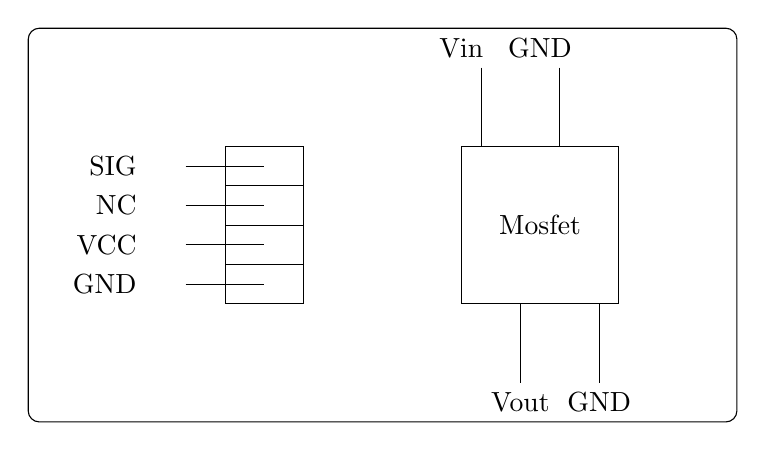
\begin{tikzpicture}
		
		
		% Rahmen des Moduls
		\draw[rounded corners] (0,0) rectangle (9,5);
		
		
		% Bereich für Grove Stecker
		\draw (2.5,1.5) rectangle (3.5,3.5);
		\draw (2.5,3.5) -- (3.5,3.5);
		\draw (2.5,3) -- (3.5,3);
		\draw (2.5,2.5) -- (3.5,2.5);
		\draw (2.5,2) -- (3.5,2);
		
		% Pins beschriften für Buchse
		\node[left] at (1.5,3.25) {SIG};
		\node[left] at (1.5,2.75) {NC};
		\node[left] at (1.5,2.25) {VCC};
		\node[left] at (1.5,1.75) {GND};
		
		% Bereich Mosfet und Spannungseingänge
		\draw (5.5,1.5) rectangle (7.5,3.5);
		
		
		
		% Pins beschriften für Spannungseingänge
		\node[above] at (5.5,4.5) {Vin};
		\node[above] at (6.5,4.5) {GND};
		\node[below] at (6.25,0.5) {Vout};
		\node[below] at (7.25,0.5) {GND};
		
		
		\node at (6.5,2.5) {Mosfet};
		
		% Detaillierte Pins und Linien
		\draw[very thin] (2,3.25) -- (3,3.25);
		\draw[very thin] (2,2.75) -- (3,2.75);
		\draw[very thin] (2,2.25) -- (3,2.25);
		\draw[very thin] (2,1.75) -- (3,1.75);
		%
		\draw[very thin] (5.75,4.5) -- (5.75,3.5);
		\draw[very thin] (6.75,4.5) -- (6.75,3.5);
		%\draw[very thin] (7.25,2.5) -- (8.25,2.5);
		\draw[very thin] (6.25,1.5) -- (6.25,0.5);
		\draw[very thin] (7.25,1.5) -- (7.25,0.5);
		
		
	\end{tikzpicture}
	\caption{Schema des Grove Mosfets nach \cite{nexperiabss138}}
	\label{fig:Mosfet-schaltplan1}
\end{figure}

\section{Pinbelegung}

In der Tabelle \ref{tab:Mosfet-connections} wird die Pinbelegung für das Mosfet mit dem Arduino beschrieben. 
\begin{table}
	\centering
	\caption{Verbindungen: Grove Mosfet-Modul zu Arduino Nano 33 BLE Sense [eigene Tabelle]}
	\label{tab:Mosfet-connections}
	\begin{tabular}{|l|l|}
		\hline
		Grove Mosfet-Modul & Arduino Nano 33 BLE Sense \\
		\hline
		SIG & Digital I/O Pin (z.B. D12, zur Steuerung des Mosfet) \\
		\hline
		NC & Nicht verbunden \\
		\hline
	    \ac{vcc} & 3.3V  \\
		\hline
		GND & GND \\
		\hline
		VIN & Spannungsquelle, Netzteil (Über Schalter) \\
		\hline
		VOUT & Verbindung zur Last (z.B. Aktor) \\
		\hline
	\end{tabular}
\end{table}



\begin{code}
	\caption{Einfaches Testprogramm Für das Mosfet nach \cite{GroveMOSFETDocs}}
	\label{Code:Mosfet}
	\ArduinoExternal{}
	{../../Code/Arduino/Mosfet/SampleGrove/SampleGrove.ino}
\end{code}

\section{Weiterführende Litaratur} 

Die folgenden Bücher befassen sich mit Leistungselektronik, insbesondere mit Mosfets in Verbindung mit Mikrocontrollern. \cite{PowEl2017} \cite{ElPArd2022}
Der nachfolgende Standard enthält die technischen Vorgaben für Halbleiterbauelemente, insbesondere für Mosfets.. \cite{IEC60747}
